\documentclass[main.tex]{subfiles}
\begin{document}

Dans la suite du chapitre on étudiera le modèle suivant : Affine en la commande
\[(\Sigma)
    \begin{cases}
      \dot{x} & = f(x) + g(x) u\\
      y & = h(x)
    \end{cases}
 \]\nopagebreak
\section{Commande par bouclage linéarisant}
\begin{figure}[H]
  \centering
  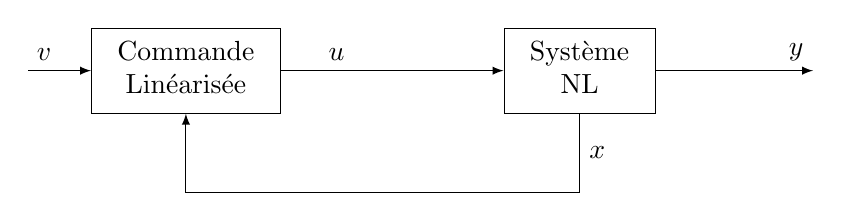
\begin{tikzpicture}
    \node[draw, minimum height=1cm] (C) at (0,0) {
      \begin{tabular}{c}
Commande\\ Linéarisée
      \end{tabular}};
    \node[draw, minimum height=1cm] (S) at (5,0) {
      \begin{tabular}{c}
Système\\ NL
      \end{tabular}};
    \draw[-latex] (-2,0) -- (C.west) node[near start,above]{$v$};
    \draw[-latex] (C.east) -- (S.west) node[near start, above]{$u$};
    \draw[-latex] (S.east) --  ++(2,0) node[above left]{$y$};
    \draw[-latex] (S.south) |- ++(-2,-1) node[near start,right]{$x$} -| (C.south);
  \end{tikzpicture}
  \caption{Principe du bouclage linéarisant}
\end{figure}
\subsection{Linéarisation entrées-sorties}
On se place dans le cas SISO: $u\in \R$ et $y\in\R$

\begin{defin}
  Le\emph{ degré relatif} $r$ du système $(\Sigma)$ est défini par $r \in \N$ tel que
  \[
    \begin{cases}

  L_gL_f^{r-1}h(x) &\neq 0\\
  L_gL_f^{k}h(x) &= 0 \quad \forall k < r-1
\end{cases}
\]
\end{defin}

\subsubsection{Procédure de linéarisation}
On cherche $r$ par le calcul des dérivées successives de $y=h(x)$ :
  \begin{align*}
    \dot{y} & = \derivp[h(x)]{x} \dot{x}\\
            & = \derivp[h(x)]{x}(f(x)+g(x)u) \\
            & = L_fh(x) + L_gh(x)u
\intertext{Si $L_gh(x)\neq0$, alors $r=1$. Sinon on continue la procédure :}
              y^{(2)} & = \derivp[L_fh(x)]{x}\dot{x} \\
            & = \derivp[L_fh(x)]{x}f(x) + \derivp[L_fh(x)]{x}g(x)u \\
            & = L^2_fh(x) + L_gL_fh(x)u
 \intertext{Si $L_gL_fh(x) \neq 0$, alors $r=2$. Sinon on continue...}
              y^{(r)} & = L_f^rh(x) + L_gL_f^{r-1}h(x)u
  \end{align*}

  \begin{rem}
  On a $1 \leq r \leq n$ car la procédure utilise la base canonique ($x_1=y,x_2=\dot{y}$) : la commande doit apparaître au maximum à la $n$-ième dérivée.
\end{rem}

  On pose $v=y^{(r)} = L_f^rh(x) + L_gL_f^{r-1}h(x)u \ne 0$ Alors:
  \[
    u  = (L_gL_f^{r-1}h(x))^{-1}(v-L_f^rh(x))
  \]

  \[
    u = \alpha(x) + \beta(x)v  , \text{ avec }
    \begin{cases}
      \alpha(x) & = -(L_gL_f^{r-1}h(x))^{-1}L_f^rh(x) \\
      \beta(x) & = (L_gL_f^{r-1}h(x))^{-1}
      \end{cases}
   \]

La nouvelle entrée de commande est $v$ telle que 
\[ \begin{cases} \dot{x} & = f(x) + g(x)\alpha(x) + g(x)\beta(x)v \\  y & = h(x) \end{cases} \]

$u = \alpha(x) + \beta(x)v$ est le bouclage linéarisant statique car à un instant fixé, la linéarisation ne dépend que de $x$ à cet instant.\\

\subsubsection{Cas $r=n$}
\begin{tabular}{c|c}
\begin{minipage}[t]{0.5\linewidth}
Choix de la base : 
\[\begin{array}{ll}
z_1 & = y = h(x) \\
z_2 & = \dot{y} = L_fh(x) \Rightarrow \dot{z_1} = z_2 \\
z_3 & = \ddot{y} = L_g^2h(x) \Rightarrow \dot{z_2} = z_3 \\
\vdots \\
y^{(n)} & = \dot{z_n} = L_f^nh(x) + L_gL_f^{n-1}h(x)u = v
\end{array}\]
\end{minipage}&
\begin{minipage}[t]{0.5\linewidth}
Nouveau modèle :
\[\begin{array}{ll}
  y & = z_1 \\
\dot{z_1} & = z_2 \\
  &\vdots \\
  &\vdots\\
\dot{z_{n-1}} & = z_n \\
\dot{z_n} & = a(z) + b(z)u = v
\end{array}\]
\end{minipage}
\end{tabular}
On a donc la commande suivante :\[ u = \frac{v-a(z)}{b(z)} \text{ avec } b(z) \neq 0 \]
Qui nécessite le changement de base des variables d'états :
\[ z = \phi(x) = \vect{\phi_1(x) \\ \vdots \\ \phi_n(x)} = \vect{ h(x) \\ L_fh(x) \\ \vdots \\ L_f^{n-1}h(x)} \]
\[ u = \alpha(x)+\beta(x)v \text{ avec } \alpha(x) = -\frac{a(z)}{b(z)}|_{z=\phi(x)} \text{ et } \beta(x) = \frac{1}{b(z)}|_{z=\phi(x)} \]

\begin{figure}[H]
  \centering
  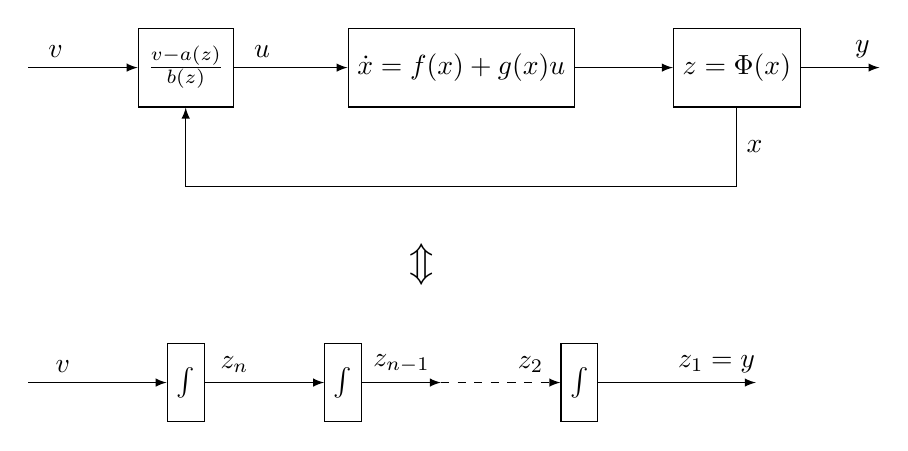
\begin{tikzpicture}
    \begin{scope}[at={(0,0)}]
    \node[draw, minimum height=1cm] (C) at (0,0) {$\frac{v-a(z)}{b(z)}$};
    \node[draw, minimum height=1cm] (S) at (3.5,0) {$\dot{x}=f(x)+g(x)u$};
    \node[draw, minimum height=1cm] (N) at (7,0) {$z=\Phi(x)$};
    \draw[-latex] (-2,0) -- (C.west) node[near start,above]{$v$};
    \draw[-latex] (C.east) -- (S.west) node[near start, above]{$u$};
    \draw[-latex] (S.east) -- (N.west);
    \draw[-latex] (N.east) --  ++(1,0) node[above left]{$y$};
    \draw[-latex] (N.south) |- ++(-2,-1) node[near start,right]{$x$} -| (C.south);
  \end{scope}
  \node at (3,-2.5){\Large$\Updownarrow$};
  \begin{scope}[shift={(0,-4)}]
    \node[draw, minimum height=1cm] (I1) at (0,0) {$\int$};
    \node[draw, minimum height=1cm] (I2) at (2,0) {$\int$};
    \node[draw, minimum height=1cm] (I3) at (5,0) {$\int$};
\draw[-latex] (-2,0) -- (I1.west) node[near start, above]{$v$};
\draw[-latex] (I1.east) -- (I2.west) node[near start, above]{$z_n$};
\draw[-latex] (I2.east) -- ++(1,0) node[midway,above]{$z_{n-1}$};
\draw[-latex,dashed] (I2.east)++(1,0) -- (I3.west) node[near end, above]{$z_{2}$};
\draw[-latex] (I3.east) -- ++(2,0) node[near end, above]{$z_1=y$};
  \end{scope}
  \end{tikzpicture}
  \caption{Forme normale}
\end{figure}

\subsubsection{Cas $r<n$}
Dans le cas ou $r < n$ il  faut ``compléter'' le système pour le rendre commandable.
\begin{align*}
  z_1 &= y\\
  z_2 &= \dot{z_1} \\
      & \vdots \\
 \dot{z_r} &= L_g^rh+L_gL_f^{r-1}h u = v
\end{align*}
Alors on  complete les variables d'état avec le vecteur$ \eta\in\R^{n-r}$ tel que:
\[
  \dot{\eta}=q(\eta,z,v,\dot{v},...)
\]
\begin{rem}
La dynamique de $\eta$ n'est pas linéaire (contrairement à $z$), pour appliquer la commande désirée il faut s'assurer que la dynamique de $\eta$ est stable car elle sera non observable par $y$.

On peux faire une analogie avec la compensation de pôles, qui n'est possible que si le pôle compensé est stable. En cachant la dynamique associée à ses poles ils ne sont plus observables
\end{rem}

\begin{rem}\emph{ À clarifier }
Ainsi on défini la dynamique des zéros. Le système commandé est en régime stationnaire :
\[
\dot{v}=0  y=0 ..
\]
La dynamique des zéro est celle $\dot{\eta} =q(\eta,0,v)$. Puisque la commande est linéaire on aussi prendre $v=0$
\end{rem}
\subsection{Dynamique des zéros}
\begin{defin}
C'est la dynamique interne pour une sortie identiquement nulle.
Ainsi, $y = 0 = z_1 \Rightarrow \dot{z_1} = \dot{z_2} = \dot{z_r} = v = 0$ et $u = -\frac{a(z)}{b(z)}$

La dynamique restante
\begin{align*}
&\left\lbrace
\begin{array}{cc}
\dot{z_{r+1}} & = q_{r+1}(z) \\
\vdots \\
\dot{z_n} = q_n(z)
\end{array}\right. \text{ où } z = (0,z_{r+1},\dots z_n)^T = (0,\text{ et }a)^T\\
& \left\lbrace
\begin{array}{cc}
\dot{\eta_1} & = q_{r+1}(0,\eta) \\
\vdots \\
\dot{\eta_{n-r}} & = q_n(0,\eta)
\end{array} \right. \text{ avec } u = \frac{-a(0,\eta)}{b(0,\eta)}
\end{align*}

\end{defin}

\begin{rem}
Si $r<n$, le système comporte une dynamique des zéros. Dans le cas ou la dynamique des zéros est instable, on peux chercher à trouver une transformation pour linéariser le modèle entrée-états, ce que l'on va étudier tout de suite.
\end{rem}


\subsection{Linéarisation entrée-états}
Dans le cas où l'on ne dispose pas d'une sortie $y=h(x)$, on essaye de trouver une sortie "fictive" grâce à un changement de variable.\\

\paragraph{Problème} : trouver le bon changement de base $z_1 = \phi_1(x)$ qui remplace $z_1=y=h(x)$ :
\[ z = \vect{z_1 \\ \vdots \\ z_n} = \vect{\phi_1(x) \\ \vdots \\ \phi_n(x)} = \phi(x) \]

$\phi$ est un difféomorphisme, i.e. bijectif et différentiable, de même pour la réciproque.\\

\begin{thm}
  Le système $\dot{x} = f(x) + g(x)u$ est \emph{linéarisable entrée-états} si
  \begin{itemize}
  \item il existe une région $\Omega \in \R^n$,où il existe un difféomorphisme $\phi:\Omega\rightarrow\R^n$
  \item il existe un retour d'état $u=\alpha(x) + \beta(x)v$ tels que le nouveau vecteur d'état est $z=\phi(x)$
    \item  la nouvelle entrée est $v$ avec $\dot{z} = Az+Bv$,
    où $A$ est la  matrice d'évolution $\in \R^{m \times n}$.
\end{itemize}
\end{thm}

En s'inspirant de la linéarisation entrée-sortie, on simplifie la recherche de $\phi(x)$ par celle de $\phi_1(x)=z_1$ et le reste des transformations est obtenu par la forme canonique (forme normale).

\begin{align*}
z_2 & = \phi_2(x) \\
& = \dot{z_1} = \dot{\phi_1}(x) \\
& = \derivp[\phi_1(x)]{x}f(x) + \derivp[\phi_1(x)]{x}g(x)u \\
& = L_f\phi_1(x) + L_g\phi_1(x)u \text{ avec } L_g\phi_1(x) = 0 \\
z_3 & = L_f^2 \phi_1(x) \text{ avec } L_gL_f\phi_1(x) = 0 \\
\phi(x) & = \vect{\phi_1(x) \\ L_f\phi_1(x) \\ \vdots \\ L_f^{n-1} \phi_1(x)} \text{ avec } L_gL_f^j \phi_1(x) = 0,\text{ et } j = 0,\dots n-2
\end{align*}

Or, $ L_gL_f^j \phi_1(x) = 0, j = 0,\dots n-2 \Leftrightarrow L_{ad_f^j g} \phi_1(x) = 0 $ car 
\begin{align*}
L_g(L_g\phi_1) - L_g(L_f\phi_1)) & = L_f(\derivp[\phi_1]{x}g)-L_g(\derivp[\phi_1]{x}f) \\
& = \derivp[^2\phi_1]{x^2}g.f + \derivp[\phi_1]{x}J_g.f - \derivp[^2 \phi_1]{x^2}g.f - \derivp[\phi_1]{x}J_f.g \\
0 & = L_{[f,g]}\phi_1 = L_{ad_f g} \phi_1 = 0
\end{align*}

Existe-t-il $\phi_1(x)$ tel que
$\begin{cases}
  L_g L_f^j \phi_1(x) & = 0, \quad j = 0, \dots, n-2\\
  L_g L_f^{n-1}  \phi_1(x) & \neq 0 \\
\end{cases} $ ?

\begin{defin}
L'application $\Delta(x)$ est une\emph{ distribution de champs de vecteurs} sur $\Omega$ si $\forall x \in \Omega, \Delta(x)$ est un sous-espace vectoriel.
\end{defin}

\begin{exemple}
\[\Delta(x) = vect \left\lbrace \vect{x_1 \\ x_2 \\2}, \vect{x_1x_3 \\ x_2x_3 \\ 2x_3},\vect{x_2 \\ x_2 \\ 0} \right\rbrace \]

\begin{align*}
x_2 = 0 & \Rightarrow \Delta(x) = vect \left\lbrace \vect{x_2 \\ 0 \\ 2} \right\rbrace \\
& \Rightarrow \Delta(x) \text{ est e.v. de dim = 1} \\
x_2 \neq 0
& \Rightarrow \Delta(x) = vect \left\lbrace \vect{x_1 \\ x_2 \\ 2},\vect{1 \\ 1 \\ 0} \right\rbrace \\
& \Rightarrow \Delta(x) \text{ est un e.v. de dim = 2}
\end{align*}
$\Delta(x)$ est une distribution de champs de vecteurs.
\end{exemple}

\begin{defin}
La distribution $\Delta$ est \emph{involutive} ssi 
\[\forall f,g \in \Delta, \quad [f,g] \in \Delta \]
\end{defin}

\begin{prop}
$\Delta(x) = \vect{f_1& \dots & f_p}$ est une distribution involutive ssi 
\[ \exists \alpha_{ij_k} : \R^n \mapsto \R \text{ tq } [f_i,f_j] = \sum_{k=1}^p \alpha_{ij_k}(x) f_k, \quad i = 1,\dots p, j = 1,\dots p\]
\end{prop}

\begin{exemple}
\[ x_2 \neq 0 \Rightarrow \Delta(x) = vect\left\lbrace \vect{x_1 \\ x_2 \\ 2}, \vect{1 \\ 1 \\ 0} \right\rbrace\]
\begin{align*}
[f_1,f_2] & = J_{f_2}f_1 - J_{f_1} f_2 \\
          & =
            \begin{bmatrix}
              0 & 0 & 0 \\
              0 & 0 & 0 \\
              0 & 0 & 0
            \end{bmatrix}
                      \vect{x_1 \\ x_2 \\ 2} -
          \begin{bmatrix}
              1 & 0 & 0 \\
              0 & 1 & 0 \\
              0 & 0 & 0
            \end{bmatrix}
  \vect{ 1 \\ 1 \\ 0} \\
& = \vect{ -1 \\ -1 \\ 0} = -f_2 \in \Delta
\end{align*}

$\Delta$ est une distribution involutive pour $x_2 \neq 0$
\end{exemple}

\newcommand{\lesys}{$\dot{x}=f(x)+g(x)u, x\in\R^n, u\in\R$}

\begin{thm}[Theoreme d'existence]
  Soit le système $\Sigma$. Il existe un changement de base $z=\phi(x)$\\[1.5em]

  linéarisant  sur $\Omega$ tel que
  \[\phi^T(x) = [\phi_1(x), L_f\phi_1(x) \dots L_f^{n-1} \phi_1(x) ]\]
  ssi :
\begin{itemize}
\item $dim(g,ad_f g, \dots ad_f^{n-1} g) = n$ (Commandabilité Kalman)
\item la distribution engendrée par $\{g, ad_f g, \dots ad_f^{n-1}g\}$ est involutive, $\forall x \in \Omega$.
\end{itemize}
%   
\end{thm}

Ainsi, la procédure de linéarisation entrée-états est réalisée via les étapes suivantes :
\begin{enumerate}
\item Construction de $E = \{ g, ad_f g, \dots, ad_f^{n-1} g \}$
\item Vérifier la commandabilité, i.e. $dim(E) = n$ (Kalman !)
\item Montrer que $\Delta(x) = vect\{E\}$ est involutif, i.e. $\exists \alpha_{ij_k}(x) : \Omega \mapsto \R$ tel que :
\[ [ad_f^i g, ad_f^j g] = \sum_{k=0}^{n-1} \alpha_{ij_k}(x).ad_f^k g, \quad i,j = 0,\dots,n-1 \]
\item Trouver $\phi_1(x)$ avec $\begin{cases}L_{ad_f^j g} \phi_1(x) & = 0, j=0,\dots n-2 \\ L_gL_f^{n-1} \phi_1(x) & \neq 0 \end{cases}$
\item Construction du nouveau vecteur d'état $z^T = \phi^T(x) = [\phi_1(x), L_f\phi_1(x) \dots L_f^{n-1} \phi_1(x) ]$
\item Linéarisation par retour d'état statique $u = \alpha(x)+\beta(x)v$, $v$ nouvelle commande du modèle linéaire, avec 
\[ \alpha(x) = -\frac{L_f^n \phi_1(x)}{L_gL_f^{n-1}\phi_1(x)} \text{ et } \beta(x) = \frac{1}{L_gL_f^{n-1}\phi_1(x)} \]
\end{enumerate}

Si le degré relatif $r<n$ dimension du modèle (entrée-sortie), alors le modèle N.L est partiellement linéarisable, mais le comportement entrée-sortie est linéaire : suffisant pour la commande du système à condition que la dynamique N.L (non linéarisée par le bouclage) est stable, i.e. $||x||$ est bornée.


Ainsi en imposant :$z_1 = y = \phi_1(x)$ le modèle est sous forme normale : 
\begin{align*}
& \left\lbrace
\begin{array}{cc}
\dot{z_1} & = z_2 \\
\vdots \\
\dot{z_r} & = v
\end{array}
\right. \text{ Partie linéaire, de dimension $r$, entrée-sortie }\\
& \left\lbrace
\begin{array}{cc}
\dot{z_{r+1}} & = q_{r+1}(z) \\
\vdots \\
\dot{z_n} & = q_n(z)
\end{array}
\right.
\text{ Partie N.L., de dimension $n-r$ n'influe sur la sortie}
\end{align*}

\begin{rem}
En linéaire, le degré relatif correspond à la différence entre le degré du dénominateur et du numérateur $r=n-m$.

En effet, $y^{(n)} + a_{n-1}y^{(n-1)} + \dots + a_1y ^{(1)} + a_0y = b_mu^{(m)} + \dots + b_1u^{(1)} + b_0u$ :
\[ \dd{}{t}\vect{x_1 \\ \vdots \\ x_n} = \left[ \begin{array}{ccccc}
0 & 1 & 0 & \dots & 0 \\
\vdots & \ddots & \ddots & \ddots & \vdots \\
\vdots & & \ddots & \ddots & 0 \\
0 & \dots & \dots & 0 & 1 \\
-a_n & -a_{n-1} & \dots & \dots & -a_1
\end{array} \right] \vect{x_1 \\ \vdots \\ x_n} + \vect{0 \\ \vdots \\ 0 \\ 1} u, y = (b_0, \dots b_m, 0 \dots 0) u\]
\begin{align*}
z_1 & = y = Cx \\
z_2 & = \dot{z_1} = C\dot{x} = C(Ax+Bu) \\
& = CAx + CBu
\intertext{ Si $r=0$, alors $CB = (b_0 \dots b_M, 0 \dots 0) ( 0 \dots 1)^T = b_m$ ($r=n-m$ zéros dans $C$)}
\intertext{ Si $CB = 0 = L_g\phi_1$,}
z_2 & = L_f \phi_1 = CAx \\
\dot{z_2} & = CA(Ax+Bu) = CA^2x + CAB u \Rightarrow r=1 (??)
\end{align*}
\end{rem}


\subsection{Système à déphasage minimal}
\paragraph{Rappel}:

  Dans le \emph{cas linéaire} le système est a déphasage minimal si les zéros sont à partie $Re<0$.



\begin{defin}
  Dans le \emph{cas non linéaire} le sytème est à déphasage minimal si dynamique des zéros stables, i.e. à l'origine on a :
\[\left\lbrace
\begin{array}{cc}
\dot{\eta_1} & = q(0,\eta) \\
\vdots \\
\dot{\eta_{n-r}} & = q(0,\eta)
\end{array} \right. \text{ est stable} \]
\end{defin}

Ainsi, quand le le système est à déphasage non minimal, on applique la linéarisation $e-s$.


\subsection{Cas MIMO du bouclage linéarisant}
\paragraph{Rappel:}
Le linéarisation revient à trouver la commande qui réalise la réciproque de la non-linéarité : problème inverse. Dans le cas où le problème est non inversible d'une manière statique (i.e. algébrique), la solution est alors de réaliser une inversion dynamique, à la manière de  l'observateur dans le cas linéaire.

Soit le système non-linéaire :
\begin{align*}
\dot{x} & = f(x) + \sum_{i=1}^m g_i(x)u_i \\
y & = \vect{k_1(x) \\ \vdots \\ k_p(x)} \text{ avec } x\in\R^n,y \in \R^p \text{ et } u=\vect{u_1 \\ \vdots \\ u_m} \in \R^m 
\end{align*} 

\begin{defin}
Le degré relatif $r$ dans le cas MIMO est défini comme $r=r_1+\dots+r_p$ si $r_i$ est le degré relatif associé à la sortie $y_i$ tel que :
\[ \forall j=1\dots m, L_{g_j}L_f^k h_i(x) = 0, \forall k < r_i-1\]
\[ \exists j =1\dots m, L_{g_j}L_f^{r_i-1} h_i(x) \neq 0\]
\end{defin}

\subsubsection{Procédure de linéarisation}
Sans perte de généralité, on pose $m=p$ (le nb de paramètre de commande est identique au nombre de sortie). Calculons les dérivées successives des sorties :
\[
\vect{ y_1^{(r_1)} \\ \vdots \\ y_p^{(r_p)}} =
\vect{ L_f^{r_1} h_1(x) \\ \vdots \\ L_f^{r_p}h_p(x) } +
\begin{bmatrix}
  L_{g_1}L_f^{r_1-1}h_1 & \dots & L_{g_m}L_f^{r_1 - 1} h_1 \\
  \vdots                     & \ddots     & \vdots                        \\
  L_{g_1}L_f^{r_p-1}    & \dots & L_{g_m}L_f^{r_p-1} h_p
\end{bmatrix}
\vect{u_1 \\ \vdots \\ u_m}
\]
On remarquera l'intérêt de poser $m=p$.

On note $D(x)$ la matrice $\R^{p\times m}$ (dite de découplage). 
\[
D(x) =
\begin{pmatrix}
L_{g_1}L_f^{r_1-1}h_1 & \dots & L_{g_m}L_f^{r_1 - 1} h_1 \\
  \vdots                     & \ddots     & \vdots                        \\
  L_{g_1}L_f^{r_p-1}    & \dots & L_{g_m}L_f^{r_p-1} h_p
\end{pmatrix}
\]



\begin{prop}
Le système MIMO est linéarisable si $r=\sum_{i=1}^p r_i = n$ avec $D(x)$ inversible.
\end{prop}



\begin{itemize}
\item Si $D(x)$ est inversible, alors la commande linéarisante est :
\[ u(x) = D(x)^{-1}( \vect{v_1 \\ \vdots \\ v_m} - \vect{L_f^{r-1} h_1(x) \\ \vdots \\ L_f^{r_p}h_p(x)}) \]
On a un bouclage ``statique''.


\item si $D(x)$ n'est pas inversible alors on introduit une dynamique pour la rendre inversible. Une méthode simple pour trouver cette dynamique est de continuer à dériver après apparition de la commande ($u_j,\dot{u}_j$).
\end{itemize}



Dans le cas où $r<n$, alors le système MIMO est partiellement linéarisable. Ainsi, $\eta$ est le vecteur d'état des $n-r$ équations non linéaires restantes.
\[ \dot{\eta} = P(z,\eta) + Q(z,\eta) u, \text{ avec } P_k(z,\eta) = L_f \eta_k \text{ et } Q_{k,j}(z,\eta) = L_{g_j}\eta_k, k = 1 \dots n-r, j = 1 \dots m \]

Ainsi la dynamique interne, i.e. dynamique des zéros
\[ \dot{\eta} = P(\underline{0},\eta)+Q(\underline{0},\eta)u(\underline{0},\eta) \text{ avec } u(\underline{0},\eta) = -D^{-1}(\underline{0},\eta)\vect{L_f^{r_1}h_1(\underline{0},\eta) \\ \vdots \\ L_f^{r_p}H_p(\underline{0},\eta)} \]

doit être stable.

Si $D(x)$ n'est pas inversible alors le bouclage linéarisant est dynamique :
\begin{align*}
u & = \alpha(x,q) + \beta(x,q) v \\
\dot{q} & = \gamma(x,q) + \delta(x,q) v
\end{align*}

tel que $z=\phi(x,q)$ est un difféomorphisme.\\

La procédure générique est de dériver $y_j$ au delà de $r_j$ pour obtenir $D(x,q)$ inversible.

Les dynamiques auxiliaires $q$ sont obtenues à partir des dérivées successives des commandes. Cette procédure est la linéarisation par bouclage dynamique.

\section{Poursuite de trajectoire asymptotique}

\subsection{Cas SISO}
Soit le système non-linéaire SISO (1) :
\[ \begin{cases} \dot{x} & = f(x,y)  \\  y & = h(x) \end{cases} \]

Il existe une trajectoire (non unique) remplaçant le vecteur d'état $x$ par $z$ les dérivées successives de la sortie $y$.

Ainsi, on peut réécrire (1) sous forme polynomiale : 
\[ P(y, \dots, y^{(n)}, u , \dots u^{(k)}) = 0 \] avec $n < \infty$ et $k< \infty$:
\[ z = \vect{ z_1 \\ \dots \\ z_n} = \vect{ y \\ \vdots \\ y^{(n-1)}} \]

Sous la condition $ \derivp[P]{y^{(n)}} \neq 0$ le modèle (1) est remplacé par la forme canonique
\begin{align*}
\dot{z_1} & = z_2\\
\vdots \\
\dot{z_n} & = C(z_1 \dots z_n, u \dots u^{(k)})
\end{align*}

On suppose la consigne $y_c$ $n$ fois dérivable par rapport au temps.

Objectif : trouver $u$ tel que $y \to y_c$ suivant une dynamique imposée.

\subsection{Procédure}
\begin{itemize}
\item On pose $\epsilon(t) = y_c(t) - y(t)$ : erreur de poursuite
\item Imposer la dynamique de poursuite : \[\epsilon^{(m)} + \beta_{m-1} \epsilon^{(m-1)} + \dots + \beta_1 \epsilon^{[1)} + \beta_0 \epsilon = 0 \] tels que $\beta_i,i=0\dots m$ sont choisis pour que le polynôme
\[ \lambda^n + \beta_{n-1} \lambda^{n-1} + \dots + \beta_1 \lambda + \beta_0 = 0 \] soit un polynone d'Hurwitz\footnote{les racines sont à parties réelles strictement négatives}.
Pour $n=m$ on a 
\[ y^{(m)} (t) = y_c^{(m)}(t) + \sum
_{i=1}^m \beta_{i-1}(y_c^{(i-1)}(t) - y^{(i-1)}(t)) \]

On peut aussi réécrire le modèle sous forme d'état $(\epsilon_1 = \epsilon)$ :
\begin{align*}
\dot{\epsilon_1} & = \epsilon_2 \\
\vdots \\
\dot{\epsilon_n} & = \hat{C}(y_c^{(n)}, Y_c, E , u , \dots
 u^{(k)}) \text{ avec } Y_c = \vect{y_c \\ \vdots \\ y_c^{(m-1)}} \text{ et } E = \vect{\epsilon_1 \\ \vdots \\ \epsilon_n}
\end{align*}

La poursuite asymptotique revient à trouver $u$ tel que 
\[\hat{C}(y_c^{(n)},Y_c,E,u,\dots u^{(k)}) = -\sum_{i=1}^n \beta_{i-1}\epsilon^{(i-1)} \Leftrightarrow C(z_1,\dots z_n,u,u^{(i)},\dots u^{(k)} = y_c^{(n)} + \sum_{i=1}^n \beta_{i-1} (y_c^{(i-1)} -z_i) \]

Dans le cas où le modèle est sous forme normale (forme obtenue pour le bouclage linéarisant) : 
\begin{align*}
 y  &= z_1\\
  \dot{z_1} & = z_2 \\
\vdots \\
\dot{z_{r-1}} & = z_r \\
\dot{z_r} & = b(z) + a(z)u \text{ avec } a(z) \neq 0 \\
\dot{z_{r+1}} & = q_{r+1} (z) \\
\vdots \\
\dot{z_n} & = q_n(z)
\end{align*}

Si $m=r$ alors \[ u = \frac{1}{a(z)} (-b(z)+y_c^{(r)} + \sum_{i=1}^r \beta_{i-1} \epsilon^{(i-1)} \]
$y_c^{(r)}$ bouclage linéarisant statique

Si $m=r+1$ alors
\[ \dot{u} = \frac{1}{a(z)} (-\dot{b}(z) - \dot{a}(z)u + y_c^{(m)} + \sum_{i=1}^m \beta_{i-1} \epsilon^{(i-1)}) \]
$\dot{a}(z)u$ bouclage linéarisant dynamique
Même démarche pour les degrés supérieurs de la poursuite asymptotique.
\end{itemize}
\begin{figure}[ht]
  \centering
  \begin{tikzpicture}
    \sbEntree{Yc}
    \sbComp{C}{Yc}
    \sbRelier[$y_c$]{Yc}{C}
    \sbBlocL{P}{
      \begin{tabular}{c}
        Commande \\ pour la \\ poursuite
      \end{tabular}
    }{C}
    \sbBlocL[4]{I1}{$\displaystyle\int$}{P}
    \sbBlocL{I2}{$\displaystyle\int$}{I1}
    \node[above] at (P-I1) {$u^{(m-r)}$};
    \node[above] at (I1-I2) {...};
    \sbBlocL{NL}{
      \begin{tabular}{c}
        Système \\ N.L
      \end{tabular}
    }{I2}
    \sbSortie{Y}{NL}
    \sbRelier[$y$]{NL}{Y}
    \sbRenvoi{NL}{P}{}
    \sbRenvoi[6]{NL-Y}{C}{}
  \end{tikzpicture}
  \caption{Commande par bouclage linéarisant}
  \label{fig:label}
\end{figure}
La difficulté de la poursuite asymptotique est la résolution de l'équation dynamique NL
\[c(z_1 \dots z_n , u \dots u^{(k)} ) y_c^{(n)} - \sum_{i=1}^m \beta_{i-1} (y_c^{(i-1)} - z_i) = 0 \]
\subsection{Système plats}

Dans le cas des systèmes plats, la solution est obtenue via les sorties plates.

\begin{defin}
  Un système est dit \emph{plat} si toutes les variables d'états $\vec{x}$  et les entrées peuvent s'écrire comme :
  \[
    \begin{cases}

      \vec{x} = \psi(y_1, ..., y_1^{(\alpha_1)}, ..., y_m,...,y_m^{(\alpha_m)}) \\
      \vec{u} = \phi(y_1, ..., y_1^{(\beta_1)}, ..., y_m,...,y_m^{(\beta_m)})
    \end{cases}
  \]
  Les $y_i$ sont alors appelées \emph{sortie plates}
\end{defin}

\begin{exemple}
Montrer que le système suivant est plat avec pour sorties plates $y_1=x_1$ et $y_2=x_2$ :
\begin{align*}
\dot{x_1} & = u_2 \\
\dot{x_2} & = x_2 + x_3u_2 \\
\dot{x_3} & = x_1u_1
\intertext{ On peut donc écrire : }
x_1 & = y_1 \\
x_2 & = y_2 \\
x_3 & = \frac{\dot{y_2-y_2}}{\dot{y_1}} \\
u_2 & = \dot{y_1}\\
u_1 & = \frac{\dot{x_3}}{y_1} = \frac{(\ddot{y_2}-\dot{y_2})\dot{y_2}-\ddot{y_1}(\dot{y_2}-y_2)}{y_3(\dot{y_1})^2}
\end{align*}
\end{exemple}

Une des utilisation des sorties est la planification simple de trajectoire. En partant de $y_i(0) = y_0 $ on souhaite arriver en un temps fini  à $y_i(T_f) = y_f$. À partir de ce cahier des charges on trouve une trajectoire ()généralement polynomiale) tel que $u = \phi(y_{1p} ... y_{1p}^{(\beta_1)},...,y_{mp},...,y_{m}^{(\beta_m)})$.

Une autre application est la résolution de l'équation N.L de la poursuite asymptotique par intégration successive de $u$.



\begin{thm}[Principe de la planification de trajectoire]
La planification peut comporter des contraintes sur la commande (énergie, saturation, ...) et sur les états (obstacles, limitation de vitesse, d'accélération...)
Pour les systèmes plats, la planification est réalisée sur les sorties plates $y\in\R^p$ et la commande est déduite par $u=\psi(y_1,\dots,y_p^{(\delta_p)})$
\end{thm}

\begin{exemple}
[Bras de robot avec $n$ degrés de libertés et $n$ actionneurs]
\[ M(q) \dot{q} + B(q,\dot{q}) = K(q,\dot{q}) u\]

$q$ : coordonnées généralisées $q\in\R^n$

$B(q,\dot{q})$ : vecteur des forces centrifuges et de Coriolis

$K(q,\dot{q})$ : matrice d'influence avec $rang(K)=n$

Le système est plat où $q\in\R^n$ sont les sorties plates.\\

La planification de trajectoire est réalisée sur les $q$, puis $u=K^{-1}(q,\dot{q})(M(q)\dot{q} + B(q,\dot{q}))$\\

On a la commande en cascade:
\[ C_0(p) = K >>1, \quad H_0(p) = \frac{H_1(p)}{1+KH_1(p)} \approx \frac{1}{K} \]
\end{exemple}
\end{document}

%%% Local Variables:
%%% mode: latex
%%% TeX-master: "main"
%%% End:
